% submission dates: https://informatics.tuwien.ac.at/study-services/dates/

\documentclass[a4paper, oneside]{discothesis}

\usepackage[utf8]{inputenc}
\usepackage[T1]{fontenc}
\usepackage{graphicx}
\usepackage{epstopdf}
\usepackage{epigraph}
\usepackage{amsmath}

\thesistype{Master's Thesis}
\title{Rethinking Adversarial Examples}

\author{Yahya Jabary}
\email{yjabary@ethz.ch}

\institute{Computer Engineering and Networks Laboratory \\[2pt] ETH Zürich}

% \logo{
\includegraphics[width=0.2\columnwidth]{figures/dsg-logo}}

\supervisors{Prof.\ Dr.\ Roger Wattenhofer\\[2pt] Prof.\ Dr.\ Schahram Dustdar}

\keywords{Robustness, Alignment, Interpretability, Algorithmic Models}
% \categories{ACM categories go here.}

\date{\today}

\setlength\parindent{0pt}

% example boxes
% https://www.overleaf.com/latex/examples/simple-stylish-box-design/stzmmcshxdng
\usepackage{mathtools}
\usepackage[many]{tcolorbox}
\usepackage{mathspec}
\usepackage{setspace}
\usepackage{multicol}
\tcbset{sharp corners, colback = white, before skip = 0.5cm, after skip = 0.5cm, breakable}
\newtcolorbox{highlightbox}{sharpish corners, boxrule = 0pt, leftrule = 4.5pt, enhanced, breakable, fuzzy shadow = {0pt}{-2pt}{-0.5pt}{0.5pt}{black!35}}
\newtcolorbox{quotebox}{sharpish corners, boxrule = 0pt, rightrule = 4.5pt, enhanced, breakable, fuzzy shadow = {0pt}{-2pt}{-0.5pt}{0.5pt}{black!35}}

\newcommand{\linebreaks}{\vspace*{0.5em}}

\usepackage{anyfontsize}
\usepackage{hyperref}
\hypersetup{colorlinks = true, linkcolor = black, urlcolor = black, citecolor = black,}
\urlstyle{same}
\makeatletter
\def\url@leostyle{%
  \@ifundefined{selectfont}{\def\UrlFont{\sf}}{\def\UrlFont{\small\ttfamily}}}
\makeatother
\urlstyle{leo}

\begin{document}

\frontmatter
\maketitle

\cleardoublepage

\begin{acknowledgements}
	This thesis comes from working on a problem that truly matters to me, in an environment where curiosity and passion were shared, and I felt a sense of belonging. The topic of adversarial examples reflects my journey well, highlighting how subtle differences in perspective can lead to vastly different interpretations and outcomes.

	I'm deeply grateful to those who supported me along the way. My parents, Shima and Florian, and my family, for their unwavering support, even when I took risks and turned down financial opportunities to pursue my passion. My partner, Laura, whose love and encouragement crossed the Atlantic and got me through many long nights.
	
	I owe much to those who made this work possible. Prof.\ Roger Wattenhofer, for trusting me with this project and guiding me with wisdom and humor. Andreas Plesner, who was just as much of a mentor as a collaborator, for his dedication to our vision. Turlan Kuzhagaliyev and Alireza Furutanpey, for their camaraderie.
	
	Thanks also to those whose paths have diverged from mine but whose impact remains with me: Prof.\ Schahram Dustdar, who enabled my studies abroad, and Prof.\ Ali Mashtizadeh, who introduced me to operating systems research.
	
	I hope to continue this journey with the same spirit that brought me here.
\end{acknowledgements}

\begin{abstract}
    % The abstract should be short, stating what you did and what the most important result is.
	% write in german and english
	...
\end{abstract}

\chapter*{Originality}
% good style: https://arxiv.org/pdf/2202.02435

I hereby declare that I have written this thesis independently, that I have completely specified the utilized sources and resources and that I have definitely marked all parts of the work - including tables, maps and figures - which belong to other works or to the internet, literally or extracted, by referencing the source as borrowed.

\section*{Papers}

\textbf{Seeing Through the Mask: Rethinking Adversarial Examples for CAPTCHAs} \\
Yahya Jabary, Andreas Plesner, Turlan Kuzhagaliyev, Roger Wattenhofer \\
\textit{ArXiv: 2409.05558}

\section*{Open source software}

The majority of time working on this thesis, was spent on developing a reproducible research pipeline for experiments in a compute and GPU memory constrained, containerized environment with compiled dependencies.

Due to the exploratory nature of the work, many of the software built and experiments conducted were not directly related to the final paper.

The following projects were developed as part of this work (in chronological order, with the most recent first):

\linebreaks

\textbf{self-ensembling} \\
All experiments related to the Self-Ensembling algorithm by Fort et al. \\
\url{https://github.com/ETH-DISCO/self-ensembling} \\
\url{https://huggingface.co/sueszli/self-ensembling-resnet152}

\linebreaks

\textbf{ensemble-everything-everywhere} \\
Pull Request: Optimizing the official Self-Ensembler repository by Fort et al. \\
\url{https://github.com/stanislavfort/ensemble-everything-everywhere/pull/2}

\linebreaks

\textbf{vision} \\
Pull Request: Containerizing TorchVision to recompile ResNet-50 from scratch. \\
\url{https://github.com/pytorch/vision/pull/8652}

\linebreaks

\textbf{advx-bench} \\
All experiments related to the geometric masks from the paper. \\
\url{https://github.com/ETH-DISCO/advx-bench} \\
\url{https://huggingface.co/sueszli/robustified_clip_vit}

\linebreaks

\textbf{cluster-tutorial} \\
Tutorial on how to circumvent the distributed NFS4 filesystem by attaching the terminal to an interactive SLURM job, run an Apptainer to enable admin privileges and redirect all filepointers to the EXT4 filesystem to avoid out-of-memory limits. A Jupyter notebook is then hosted on a public IP address. \\
\url{https://github.com/ETH-DISCO/cluster-tutorial}

\linebreaks

\textbf{python-template} \\
Short scripts to \texttt{pip-compile} dependencies, containerize the environment and translate back and forth between Conda and Docker for different job submission systems. \\
\url{https://github.com/sueszli/python-template/}

\linebreaks

\textbf{captcha-the-flag} \\
Cybersecurity emulation for CAPTCHAs: A deployable replica of Google's reCAPTCHAv2 and a scraper used to evaluate challenges against solvers. \\
\url{https://github.com/ETH-DISCO/captcha-the-flag}

\section*{Breakdown of contributions}

For the paper, Andreas Plesner had the original idea. The written text was joint work between all authors, with Prof.\ Roger Wattenhofer taking the lead on creating a cohesive narrative for our experiments, Andreas and me writing the majority of the text, and Turlan providing experimental results and feedback. The TU Wien DSG lab kindly provided the computational resources for robustifying a ResNet-50 model, which unfortunately did not make it into the final version of the paper. Additionally, Alireza Furutanpey suggested using LPIPS as a metric to evaluate the perceptual quality of adversarial examples, which we incorporated into our weighted objective function.

Regarding the developed software, all contributions are my own, unless stated otherwise in the repository. A prototype of the self-ensembled ResNet-50 model was developed by Andreas Plesner, but the authors soon released their own implementation, which was then used in all experiments for consistency.

Andreas Plesner diligently proofread this manuscript for errors. As is traditional, any errors that remain are of course mine alone.

\tableofcontents

\mainmatter

\chapter{Introduction}

We have two goals in writing this document. One: fulfilling the requirements for a master's degree by presenting and extending our original research~\cite{jabary2024seeing} in thesis form. Two: offering a fresh and cohesive perspective on the rapidly evolving and, in our view, really exciting field of adversarial machine learning to a broader audience, with fewer technical prerequisites. We hope it will be valuable to those interested.

\section{Definition}

Adversarial examples are closely related to the concept of perturbation methods\footnote{Thanks to Prof.\ Roger Wattenhofer for sharing this piece of unorthodox history.}.

The origin of perturbations can be traced back to the early days of computational geometry by Seidel et al. in 1998~\cite{seidel1998nature}. Perturbation techniques in computational geometry address a fundamental challenge: handling ``degeneracies'' in geometric algorithms. These are special cases that occur when geometric primitives align in ways that break the general position assumptions the algorithms rely on.

\begin{highlightbox}
	\textbf{Example:} Perturbation scheme for a Linear Classifier \\

	Consider a simple case of determining whether a point lies above or below a line~\cite{de2000computational}. While this classification appears straightforward, numerical issues arise when the point lies exactly on the line. Such degeneracies can cascade into algorithm failures or inconsistent results. The elegant solution is to imagine slightly moving (perturbing) the geometric objects to eliminate these special cases. Formally, we can express symbolic perturbation as $p_\varepsilon(x) = x + \varepsilon \cdot \delta(x)$ where $x$ is the original input, $\varepsilon$ is an infinitesimally small positive number the exact value of which is unimportant, and $\delta(x)$ is the perturbation function to break degeneracies. \\

	A perturbation scheme should be (1) consistent, meaning that the same input always produces the same perturbed output (2) infinitesimal, such that perturbations are small enough not to affect non-degenerate cases and (3) effective, in breaking all possible degeneracies. \\

	One powerful perturbation approach is Simulation of Simplicity (SoS)~\cite{franklin2022implementing, edelsbrunner2002topological, edelsbrunner2001sink, edelsbrunner1990simulation, levy2016robustness, schorn1993axiomatic}. SoS systematically perturbs input coordinates using powers of a symbolic infinitesimal. For a point $p_i = (x_i, y_i)$, the perturbed coordinates become:

	$$(\tilde{x_i}, \tilde{y_i}) = (x_i + \varepsilon^{2i}, y_i + \varepsilon^{2i+1}) = p_i + \varepsilon^{2i} \cdot (1, \varepsilon)$$

	This scheme ensures that no two perturbed points share any coordinate, effectively eliminating collinearity and other degeneracies.
\end{highlightbox}

The beauty of perturbation methods lies in their ability to handle degeneracies without explicitly detecting them, making geometric algorithms both simpler and more robust.

Adversarial examples on the other hand, first introduced by Szegedy et al.\ in 2014~\cite{szegedy2013intriguing}, follow the same principles as perturbation methods, but with the opposite objective. Instead of seeking to eliminate degeneracies (brittleness in the decision boundary), they exploit them to cause targeted misclassifications. Intuitively they can be understood as seeking the closest point in the input space that lies on the ``wrong side'' of a decision boundary relative to the original input. This shift, applied to the original input, creates an adversarial example.

\begin{highlightbox}
	\textbf{Example:} Fast Gradient Sign Method (FGSM) \\

	FGSM is one of the earliest and most widely recognized adversarial attack techniques, introduced by Goodfellow et al.~\cite{goodfellow2014explaining} in the context of visual recognition tasks. Given an input image $x$, FGSM generates an adversarial example $x'$ by perturbing the input in the direction of the gradient of the loss function with respect to the input.\\

	The perturbation is controlled by a parameter $\varepsilon > 0$~\footnote{Commonly $\varepsilon = 8/255$ for 8-bit images, so it stays within the precision constraints of the pixel values.}, which determines the magnitude of the change based on the direction of change for each pixel or feature in the input $x$. The model's loss function denoted by $J$, $\theta$ represents the model's parameters, and $y$ is the true target label. \\
	
	It works by calculating the gradient of the loss function with respect to the input, $\nabla_x J(\theta, x, y)$, and then adjusting the input in the direction of this gradient. The sign of the gradient, $\text{sign}(\nabla_x J(\theta, x, y))$, is used to ensure that the perturbation is small, while the $\ell_\infty$-norm constraint ensures that the change to the input remains ``imperceptible'' to human observers~\cite{goodfellow2014explaining, zhang2019adversarial}. More on the concept of imperceptibility later.\\
	
	The process for generating an adversarial example with FGSM can be expressed as:
	
	$$x' = x + \underbracket{\varepsilon \cdot \text{sign}(\nabla_x J(\theta, x, y))}_{\text{Perturbation}}$$
	
	In the untargeted version, the perturbation is designed to increase the loss for the correct class. In the targeted version the perturbation is designed to minimize the loss with respect to the adversary's chosen target class, making the model predict it deliberately.
\end{highlightbox}

While initially discovered in computer vision applications, the attack can be crafted for any domain or data type, even graphs~\cite{Kashyap2024AdversarialAA}. Natural language processing models can be attacked by circumventing the discrete nature of text data~\cite{Han2022TextAA, meng2020geometry, yang2024assessing}. Speech recognition systems are vulnerable to audio-based attacks, where crafted noise can cause system failure~\cite{rajaratnam2018noise}. Deep reinforcement learning applications, including pathfinding and robot control, have also shown susceptibility to adversarial manipulations that can compromise their decision-making capabilities~\cite{Bai2018AdversarialEC}.

\section{Threat Modeling}

Having established the general concept of adversarial examples, we can now explore the various ways they can be categorized. Our system is not exhaustive: The field continues to evolve, with new attack vectors emerging regularly~\cite{Khaleel2024AdversarialAI}. This is particularly important in threat modeling, where the goal is to anticipate and defend against potential attacks.

We can differentiate between white-box and black-box attacks. White-box attacks assume complete knowledge of and access to the target model, while black-box attacks operate with limited or no access to the model's internal workings~\cite{capozzi2024adversarial}. Interestingly, research has shown that in some cases, black-box attacks can be more effective than white-box approaches at compromising model security~\cite{capozzi2024adversarial}.

An attack can be targeted or untargeted. Targeted attacks aim to manipulate the model into producing a specific, predetermined output, whereas untargeted attacks simply seek to cause any misclassification or erroneous output~\cite{capozzi2024adversarial, Kashyap2024AdversarialAA}. This distinction is particularly relevant in security-critical applications, where the attacker's goals may vary from causing general disruption to achieving specific malicious outcomes.

The method used to generate adversarial examples can be gradient-based, optimization-based or search-based strategies. For example, some text-based attacks leverage language models to generate alternatives for masked tokens, ensuring grammatical correctness and semantic coherence~\cite{garg2020bae}.

The extent to which adversarial examples are transferable \textendash{} meaning their ability to fool multiple different models \textendash{} is another way to differentiate them. Some adversarial examples demonstrate high transferability across various model architectures, while others are more model-specific in their effectiveness~\cite{Li2022ASO, li2022review}. Recent research has shown that adversarial examples are more readily transferable between vanilla neural networks than between defended ones~\cite{li2019nattack, zheng2023black}.

Finally, the attacks can be either focused on preserving the semantic meaning of inputs or exploit the mathematical properties of models without regard for semantic interpretation provides~\cite{browne2020semantics}.

\section{Imperceptible $\not=$ Semantics Preserving}

Adversarial examples are traditionally expected to have two key properties: (1) they should successfully cause misclassification in machine learning models while (2) remaining imperceptible to human observers~\cite{cubuk2017intriguing}.

However, the concept of ``imperceptibility [to humans]'' as originally proposed by Szegedy et al.~\cite{szegedy2013intriguing} by limiting pixel-space perturbations through an $\varepsilon$-bounded constraint is fundamentally flawed. This is because the human visual system is not solely reliant on pixel-space information to interpret images~\cite{ ning2023hflic}:

\begin{figure}
    \centering
    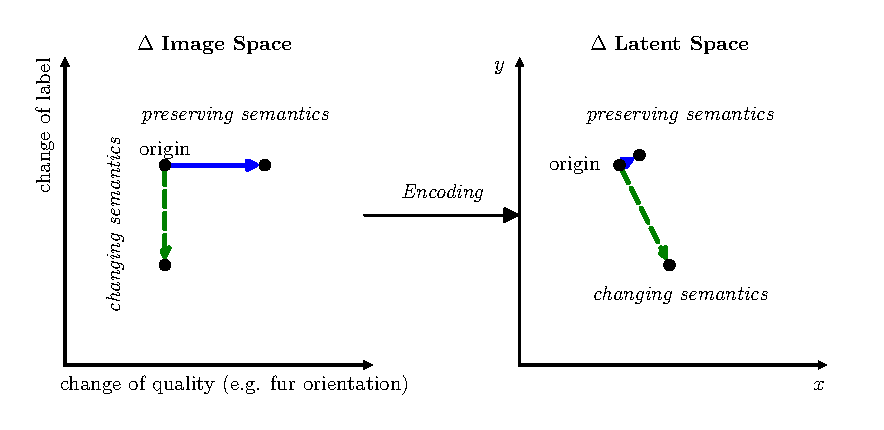
\includegraphics[width=1\columnwidth]{figures/latentspace.pdf}
    \caption{Semantics preserving/changing perturbations in pixel/latent-space.}
    \label{fig:latentspace}
\end{figure}

\begin{enumerate}
	\item \textit{Changing many pixels doesn't necessarily change semantics}: For instance, changes in lighting, exposure, sharpness, field of view or even the the orientation of an animal's fur~\cite{kilcher2021dimpled} does not necessarily alter the semantic content of an image, despite involving many pixel-space changes. The figure~\ref{fig:latentspace} serves to illustrate this point, assuming that the latent representations are perfectly aligned with the human judgement function.

	\item \textit{Changing few pixels doesn't necessarily preserve semantics}: The assumption that minimal pixel-space changes ensure semantic preservation is also flawed. This is because small $\varepsilon$-bounded adversarial perturbations are found to cause misclassification in time-constrained humans~\cite{elsayed2018adversarial}. Even more interestingly, humans detect forged low-$\varepsilon$ adversarial examples with high accuracy in both the visual (85.4\%)~\cite{veerabadran2023subtle} and textual ($\geq$70\%)~\cite{herel2023preserving} domain. Invertible neural networks can partially mitigate this issue in the visual domain~\cite{chen2023imperceptible}.
\end{enumerate}

\begin{highlightbox}
	\textbf{Open Question:} If imperceptibility is not a reliable indicator of semantic preservation, then what are the true properties of adversarial examples?
\end{highlightbox}

Recent research has shifted towards more nuanced concepts like ``semantic preservation''~\cite{careil2023towards} acknowledging that the relationship between perturbation size and semantic change is not straightforward. This shift has led to the development of new methods for generating adversarial examples that focus on preserving semantic information rather than relying on pixel-space constraints~\cite{lee2020semantics}.

The challenge of defining semantics remains central to this discussion. Without perfect representations that align with human judgment functions, we must rely on the best available encoders as proxies for semantic preservation~\cite{herel2023preserving}. This pragmatic approach acknowledges the limitations of current technology while striving for more meaningful adversarial examples.

\section{Inner Representations}

The internal latent representations of neural networks, their alignment with human understanding and the resuling gap between the two (the human-machine vision gap~\cite{geirhos2021partial}) is a central theme in adversarial machine learning research. This gap has many practical implications for the robustness and interpretability of machine learning models.

Neural networks trained with topological features develop substantially different internal representations compared to those trained on raw data, though these differences can sometimes be reconciled through simple affine transformations~\cite{mcguire2023neural}. This finding suggests that while the structural representations may differ, the underlying semantic understanding might be preserved across different training approaches.

The Centered Kernel Alignment (CKA) metric enables us to compare neural network representations, though it comes with important caveats. In biological and artificial neural networks, CKA can show artificially high similarity scores in low-data, high-dimensionality scenarios, even with random matrices~\cite{murphy2024correcting}. This limitation is particularly relevant when comparing representations of different sizes or when analyzing specific regions of interest.

The relationship between network architecture and concept representation has also been explored. Generally higher-level concepts are typically better represented in the final layers of neural networks, while lower-level concepts are often better captured in middle layers~\cite{Agafonov2022AnEO, Agafonov2022LocalizationOO}. This hierarchical organization mirrors our understanding of human cognitive processing and suggests that neural networks naturally develop structured representations that align with human conceptual understanding.

The choice of objective function significantly influences how networks represent information, particularly when dealing with biased data. Networks trained with Negative Log Likelihood and Softmax Cross-Entropy loss functions demonstrate comparable capabilities in developing robust representations~\cite{bangaru2022interpreting}.

Recent research~\cite{bansal2021revisiting} has demonstrated that neural networks with strong performance tend to learn similar internal representations, regardless of their training methodology. Networks trained through different approaches, such as supervised or self-supervised learning, can be effectively ``stitched'' together without significant performance degradation. This suggests a convergence in how successful neural networks represent information.

This aligns with the ``Platonic Representation Hypothesis''~\cite{huh2024platonic}, which suggests that neural networks are converging toward a shared statistical model of reality, regardless of their training objectives or architectures. As models become larger and are trained on more diverse tasks and data, their internal representations increasingly align with each other, even across different modalities like vision and language. This convergence appears to be driven by the fundamental constraints\footnote{Formally: ``If an optimal representation exists in function space, larger hypothesis spaces are more likely to cover it.''} of modeling the underlying structure of the real world, similar to Plato's concept of an ideal reality that exists beyond our sensory perceptions. The hypothesis proposes that this convergence is not coincidental but rather a natural consequence of different models attempting to capture the same underlying statistical patterns and relationships that exist in reality~\cite{huh2024platonic}. 

Should the ``Platonic Representation Hypothesis'' hold true, this would either mean that (a) adversarial examples as we know them are misalignments from a converged model of reality, or (b) that there exist a universal adversarial example that can fool any model, regardless of its architecture, training data or objective function, converging to a single and shared model of reality.

Recent work by Moosavi-Dezfooli et al.\ \cite{moosavi2017universal} have demonstrated the existence of a single perturbation that can fool most models for all naturally occurring images, adding weight to the latter interpretation, though the question remains open.

\section{Open Questions \& Mental Models}

The question discussed in the previous section is just one of many that remain open and yet have to be fully explained~\cite{shamir2021dimpled}. Among them are:

\begin{itemize}
	\setlength\itemsep{0em}
	\item What are adversarial examples?
	\item Why are the adversarial examples so close to the original images?
	\item Why don't the adversarial perturbations resemble the target class?
	\item Why do robustness and accuracy trade-off~\cite{zhang2019theoretically}?
	\item Why do adversarial examples transfer between models, even on disjoint training sets~\cite{szegedy2013intriguing}?
	\item Why do adversarial examples transfer between models~\cite{szegedy2013intriguing}?
	\item Why do adversarial examples transfer between models and time-limited humans~\cite{elsayed2018adversarial}?
\end{itemize}

Initially, when Szegedy et al.\ \cite{szegedy2013intriguing} coined the term they proposed that adversarial examples are caused by (1) neural networks developing internal representations that become increasingly disconnected from the input features as they progress through deeper layers, and (2) that these networks fail to maintain the smoothness properties typically assumed in traditional machine learning approaches. The idea was that this lack of smoothness gives them their expressive power, but also makes them vulnerable to these attacks.

\begin{highlightbox}
	\textbf{Definition:} Manifold \\
	
	The first attempt to explain adversarial examples used the term ``manifold''. It refers to a data submanifold.
	
	\begin{flushright}
		\textit{``In some sense, what we describe is a way to traverse the manifold represented by the network [...]. The adversarial examples represent low-probability (high-dimensional) `pockets' in the manifold [...].''}
		
		\textemdash{} Szegedy et al., 2013~\cite{szegedy2013intriguing}
	\end{flushright}	
	
	A manifold can be thought of as a low-dimensional structure embedded in a high-dimensional space, representing the set of valid data points (e.g., natural images) that the neural network is trained to classify. Mathematically, if the input data lies on a manifold $\mathcal{M} \subset \mathbb{R}^m$, then $\mathcal{M}$ represents the subset of the high-dimensional input space $\mathbb{R}^m$ that corresponds to meaningful or real-world data. \\

	Szegedy et al.\ suggest that adversarial examples exploit the structure of this manifold and its surrounding space. Specifically, adversarial examples are small perturbations $r$ added to an input $x \in \mathcal{M}$, such that the perturbed input $x' = x + r$ lies off the data manifold but still within the high-dimensional input space. \\
	
	Formally, given a classifier $f: \mathbb{R}^m \to \{1, ..., k\}$ and its associated loss function $\text{Loss}_f(x, y)$, an adversarial example $x'$ for an input $x$ with true label $y$ can be found by solving:
	
	$$\min_{r} \|r\|_2 \quad \text{subject to } f(x + r) \neq y, \; x + r \in [0, 1]^m$$
	
	where $r$ is constrained to be small (e.g., in terms of its $L_2$-norm). This optimization problem effectively traverses the space near $x$, moving off the manifold $\mathcal{M}$, to find regions where the classifier's decision boundary behaves unexpectedly. \\
	
	The paper suggests that these adversarial examples expose ``blind spots'' in the learned representation of the manifold by the neural network. The network's decision boundary may extend into regions near $\mathcal{M}$ in ways that are not semantically meaningful, allowing adversarial perturbations to exploit these regions. This phenomenon arises due to the high dimensionality of the input space and the discontinuous mappings learned by deep networks, which can fail to generalize smoothly beyond the manifold~\cite{khoury2018geometry, Jha2018DetectingAE, Sha2020ADA, dube2018high, shamir2021dimpled}. \\
	
	A more rigorous definition of the manifold hypothesis is provided by Khoury et al.\ ~\cite{khoury2018geometry}.
\end{highlightbox}

\begin{highlightbox}
	\textbf{Definition:} Realism  \\

	A ``realistic subspace'' can be understood as a subset of the data manifold where the images appear plausible according to human perception or a given distribution $P$. A simple formula that expresses this idea elegantly to quantify realism is derived from the notion of randomness deficiency in algorithmic information theory~\cite{theis2024makes}:

	$$U(x) = -\log P(x) - K(x)$$

	where $P(x)$ is the probability density of the image $x$ under the target distribution, and $K(x)$ is the Kolmogorov complexity of $x$, representing the shortest description of $x$ in a universal programming language. This measure, called a ``universal critic'', captures how well $x$ aligns with both the statistical properties of $P$ and its compressibility. A low value of $U(x)$ indicates that $x$ is realistic, while a high value suggests it is unrealistic~\cite{theis2024makes}. \\

	This approach generalizes prior methods by integrating both probabilistic and structural aspects of realism. It highlights that realism depends not only on adherence to statistical patterns (e.g., probabilities or divergences) but also on whether an image can be plausibly generated within the constraints of $P$. While directly computing $K(x)$ is infeasible due to its uncomputability, practical approximations (e.g., compression algorithms or neural network-based critics) can serve as proxies~\cite{theis2024makes}. \\

	The distinction between realistic and unrealistic perturbations is crucial for practical applications, as some adversarial examples may be mathematically valid but physically impossible to realize in real-world scenarios~\cite{dyrmishi2023empirical}. \\
	
	The challenge of quantifying realism remains a fundamental problem in machine learning~\cite{theis2024makes}.
\end{highlightbox}

Since then there have been many attempts at finding a cohesive narrative to explain these counter-intuitive properties, each with their own limitations and assumptions \textendash{} some complementary, some contradictory~\cite{ilyas2019adversarial}.

\paragraph{Non-robust features \& concentration of measure in high-dimensions.} Most popularly, Ilyas et al.\ \cite{ilyas2019adversarial} proposed that features that models learn from can be divided in 3 categories: (1) useless featurs, to be discarded by the feature extractor, (2) robust features, which are comprehensible to humans, generalize across multiple datasets and remain stable under small adversarial perturbations, and (3) non-robust features, which are incomprehensible to humans, learned by the supervised model to exploit patterns in the data distribution which are highly effective for the task at hand but also brittle and easily manipulated by adversarial perturbations. The authors suggest that the vulnerability of deep neural networks to adversarial examples is due to their reliance on non-robust features, and inherent to how the models are optimized to minimize the loss function. In essence, the authors argue that adversarial vulnerability is a property of the dataset, not the algorithm and by removing these non-robust features from the training data although the adversarial robustness of the model can be improved, due to information loss of the most predictive features, the model's overall accuracy will decrease. This view is also shared among~\cite{engstrom2019a, raghunathan2018certified, wong2018provable, xiao2018training, cohen2019certified, fawzi2018adversarial, mahloujifar2019curse, shafahi2018adversarial, gilmer2018adversarial, madry2017towards}.

\paragraph{Theoretical constructions which incidentally exploit non-robust features.} A complimenting hypothesis is that because models trained to maximize accuracy will naturally utilize non-robust data, regardless of whether it aligns with human perception~\cite{ilyas2019adversarial} they add a low-magnitude weight to sensitive variables that can get overamplified by adversarial examples~\cite{bubeck2019adversarial, nakkiran2019adversarial}. The assumption is that this happens due to computational constraints or model complexity.

\paragraph{Insufficient data.} Schmidt et al. argue~\cite{schmidt2018adversarially} that adversarial vulnerabilities are intrinsic to statistical learning in high-dimensional spaces and not merely due to flaws in specific algorithms or architectures. This is a natural consequence of the mental model proposed by Ilyas et al.\ \cite{ilyas2019adversarial}. They also argue that due to information loss in a robust dataset, significantly more data is required during training in order to achieve comparable performance.

\paragraph{Boundary Tilting.} A competing view by Tanay and Kim et al.\ \cite{tanay2016boundary,kim2019bridging} suggests that adversarial examples exist because decision boundaries extend beyond the actual data manifold and can lie uncomfortably close to it, essentially viewing adversarial examples as a consequence of overfitting. This observation can be quantified through the concept of adversarial strength, which relates to the angular deviation between the classifier and the nearest centroid classifier. The authors also argue that this vulnerability can be addressed through proper regularization techniques.

\paragraph{Test Error in Noise.} There might be a link between robustness to random noise and adversarial attacks~\cite{fawzi2016robustness, ford2019adversarial, lecuyer2019certified, cohen2019certified, ford2019adversarial}. This might imply that adversarial examples exploit inherent weaknesses in how models generalize under noisy or perturbed conditions.

\paragraph{Local Linearity.} Goodfellow, Shlens, and Szegedy et al.\ \cite{goodfellow2014explaining, madry2017towards} argue that even though DNNs are highly nonlinear overall, their behavior in high-dimensional spaces often resembles that of linear models. This makes the models vulnerable to small, targeted perturbations similar to how they're computed by FGSM. However some adversarial examples are successful all while defying the assumption of local linearity and reducing a model's linearity does not necessarily improve its robustness either~\cite{athalye2018obfuscated}.

\paragraph{Piecewise-linear decision boundaries.} In the complementary \textit{dimpled manifold hypothesis}~\cite{shamir2021dimpled} the central claim is that adversarial examples emerge because we attempt to fit high $n-1$ dimensional decision boundaries to inherently low-dimensional data like images (which can be losslessly projected to $k \ll n$ dimensions). This leaves redundant dimensions on which adversarial examples won't be judged, which enables them exist roughly perpendicularly from the true location of the low-dimensional natural image, by using large gradients. Additionally the authors differentiate between on-manifold and off-manifold adversarial examples, based on the angle of the gradients relative to the data manifold.

The authors suggest that decision boundaries of neural networks evolve during training. This happens through two distinct phases: First, there is a rapid ``clinging'' phase where the decision boundary moves close to the low-dimensional image manifold containing the training examples. This is followed by a slower ``dimpling'' phase that creates shallow bulges in the decision boundary, pushing it to the correct side of the training examples, without shifting the plane. This natural process based on gradient descent is highly efficient, but it also leaves a brittle decision boundary that can be easily exploited.

This implies that any attempt to robustify a network by limiting all its directional derivatives will make it harder to train and thus less accurate.

It also explains why networks trained on incorrectly labeled adversarial examples can still perform well on regular test images, as the main effect of adversarial training is simply to deepen these dimples in the decision boundary.

Lukas Karner successfully reproduced the experiments from the ``Dimpled Manifold Hypothesis'' paper in 2023 and demonstrated that dimensionality reductions increases the interpretability of the perturbations to humans~\cite{karner2023dimpled}.

However, most likely despite the experiments carried out being correct in themselves, the chain of reasoning might be flawed, as shown by a succinct counterexample by Yannik Kilcher in 2021 in less than 100 lines of code~\cite{kilcher2021dimpledcode, kilcher2021dimpled}. While the ``Dimpled Manifold Hypothesis'' implies a relatively uniform vulnerability across all dimensions the counterexperiment contradicts these assumptions through successful adversarial attacks constructed by perturbing either an arbitrary subset of selected dimensions or their complement. If the decision boundary truly ``clung'' to the data manifold, restricting perturbations to a subset of dimensions would not have produced successful adversarial examples. The ability to generate adversarial examples in complementary subspaces suggests the decision boundary structure is more complex than just simple dimples.

\section{Countermeasures}


% - adversarial training (kind of like distillation)

% different architectures:
% - robustness with guarantees: https://arxiv.org/pdf/2404.13631v1
% - self-ensembling architecture (state of the art)







\newpage

\chapter{Motivation}

Finally, having discussed the theory behind adversarial examples, we can now turn our attention to the practical implications of these attacks. Adversarial examples have been shown to be effective in a wide range of applications, from computer vision to natural language processing to reinforcement learning. They have been used to fool state-of-the-art models, including those used in security-critical applications such as malware detection and autonomous driving. As a result, researchers and practitioners are increasingly interested in developing robust machine learning models that can withstand adversarial attacks.

% interpretability - baking adversarial robustness right into model
% - 

% cybersecurity - adversarial examples in the wild
% - One particularly entertaining example is the subversion of the conference paper-reviewer assignment model by Eisenhofer et al.~\cite{eisenhofer2023no}, where authors preselect reviewers to gain a competitive advantage. 
% - fooling any kind of detection systen: malware detection, supply chain attacks, tax evasion, etc.
% - using adversarial examples as a turing test for captchas, particularly interesting because the "perceptual quality" part can take care of itself by gathering data from deployment




\chapter{Methodology}

\section{Geometric masks inspired by hCaptcha}

\section{Self-ensembled learning}



\chapter{Results}


% \begin{theorem}[First Theorem] \label{thm:first theorem}
% 	This is our first theorem.
% \end{theorem}

% \begin{proof}
% 	And this is the proof of the first theorem with a complicated formula and a reference to Theorem \ref{thm:first theorem}. Lorem ipsum dolor sit amet, consetetur sadipscing elitr, sed diam nonumy eirmod tempor invidunt ut labore et dolore magna aliquyam erat, sed diam voluptua. Lorem ipsum dolor sit amet, consetetur sadipscing elitr, sed diam nonumy eirmod tempor invidunt ut labore et dolore magna aliquyam erat, sed diam voluptua.
% 	\begin{equation}
% 		{\frac {\mathrm d}{\mathrm dx}}\arctan(\sin({x}^{2}))=-2 \cdot {\frac {\cos({x}^{2})x}{-2+\left (\cos({x}^{2})\right )^{2}}}
% 	\end{equation}	
% \end{proof}

\chapter{Summary}

\begin{flushright}
	\textit{``The stuff is what the stuff is, brother. Okay. We don't ask questions about the weights. We just wake up, we go to work, we use the weights, we go back home. Okay. If we change the weights, the predictions would be different and less good, probably... depending on the weather... so we don't ask about the weights.''}
	
	\textemdash{} James Mickens, USENIX Security 18 Opening Keynote~\cite{218395}
\end{flushright}

\bigskip










\bibliographystyle{IEEEtran}
\bibliography{references}

% \appendix
% \chapter{Appendix: Overview of Generative AI Tools Used}

% Note: This appendix is a mandatory part of the thesis.

% Generative language models were used to assist in the writing of this thesis. The following tools were used to generate text, which was then manually reviewed and edited for clarity and coherence:

% \begin{itemize}
% 	\item JetBrains Grazie (version: 16 October 2024) - Spell and grammar checking
% 	\item Google Translate (latest version as of December 2024) - Translations
% 	\item GitHub Copilot (latest version as of December 2024) - Text completion
% 	\item Perplexity.AI (latest version as of December 2024) - Retrieval Augmented Generation, combined with Claude Sonnet 3.5 and OpenAI o1
% \end{itemize}

% The exact prompts used for each tool are not available, as they were generated interactively during the writing process.

\end{document}
